\documentclass[12pt]{article}
 \usepackage[margin=1in]{geometry} 
\usepackage[utf8]{inputenc}
\usepackage{graphicx}
\usepackage{caption}
\usepackage{listings}
\usepackage{blindtext}
\usepackage{float}
\usepackage{amsmath}
\usepackage{amsfonts}
\usepackage{amssymb}
\usepackage{amsmath,amsthm,amssymb,amsfonts}
%for raman ciphers:
\makeatletter
\newcommand*{\rom}[1]{\expandafter\@slowromancap\romannumeral #1@}
\makeatother
%end
 
\newcommand{\N}{\mathbb{N}}
\newcommand{\Z}{\mathbb{Z}}
 
\newenvironment{problem}[2][Problem]{\begin{trivlist}
\item[\hskip \labelsep {\bfseries #1}\hskip \labelsep {\bfseries #2.}]}{\end{trivlist}}
%If you want to title your bold things something different just make another thing exactly like this but replace "problem" with the name of the thing you want, like theorem or lemma or whatever
 
\begin{document}
 
%\renewcommand{\qedsymbol}{\filledbox}
%Good resources for looking up how to do stuff:
%Binary operators: http://www.access2science.com/latex/Binary.html
%General help: http://en.wikibooks.org/wiki/LaTeX/Mathematics
%Or just google stuff
 
\title{Assignment \rom{3} \\
\large Numerical Methods} 
%\subtitle{Numerical Methods}
\author{T.J. Oosterhuis}
\maketitle
%
\section*{Exercise \rom{1}}
%how should the function be called + example
The function Oosterhuis\_assignment3\_exercise1 uses the least squares of residuals method to give a function that is an approximation of the data. The input is a bivariate dataset and a vector of initial gusses for $\lambda_1,..,\lambda_m.$ An example are the arguments 'data3' and the vector $\begin{bmatrix} \lambda_1 && \lambda_2 && \lambda_3 && \lambda_4 \end{bmatrix} =  \begin{bmatrix} 0.1 && 0.2 && 0.3 && -0.2 \end{bmatrix}$, where data3 is a bivariate dataset. The output of the function with these inputs is a vector $\lambda = \begin{bmatrix} -0.13 && 0.84 && -0.86 && -0.39 \end{bmatrix}$, a vector $C = \begin{bmatrix} 0.32 && -0.11 && 0.01 && 0.35 \end{bmatrix}$  and third the sums of the squared residues which is $59.90$.

%short discussion of the reliability and precision of the answer. restrictions program. When does program not work?
The reliability and precision of the computed lambdas, values voor $C$ and the residue depends on the user input. When the initial guesses for lambdas are 'bad', the function can return a approximation for the data that fits the data quite bad. This is for example the case when for the dataset data3 the initial guesses for the lambdas don't contain a negative value. The plot of such an result is shown in figure \ref{ex1_badplot}. We see the sum of the squared residues is $76.10$, which is also much higher than in the example above when a negative intial guess was used for one of the lambdas.
\begin{figure}[H]
\centering
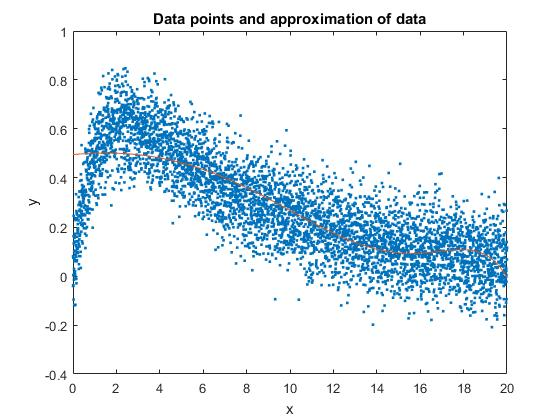
\includegraphics[width=0.6\linewidth,natwidth=610,natheight=642]{ex1_badplot.jpg}
%[width=0.6\linewidth]
%\caption{Data and approximation for dataset 'data3', using $\lambda = \begin{bmatrix} 0.10 && 0.20 && 0.30 && 0.15 \end{bmatrix}$}
\label{ex1_badplot}
\end{figure}

%illustration of output and how figure was produced. describe picture
Figures 1 to 4 show the solution of the least square approximation along with the data points for four different data sets. This output was produced by first plotting the data and then plotting the independent variables against the solution of $A * C$, where the matrix A and the vector C both depent on the new values for the lambdas.
%PLAATJES
\begin{figure}[H]
\parbox[t]{0.4\textwidth}{
	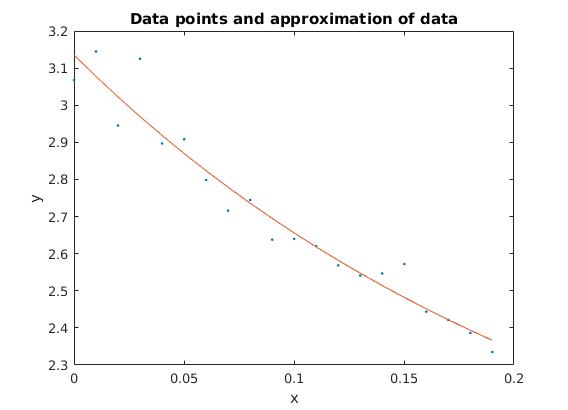
\includegraphics[width=\linewidth,natwidth=610,natheight=642]{ex1_testdata.jpg}
	\caption{Data and least square approximatiotn for 20 data points.}
    %\label{normaal}
}
\hfill
\parbox[t]{0.4\textwidth}{
	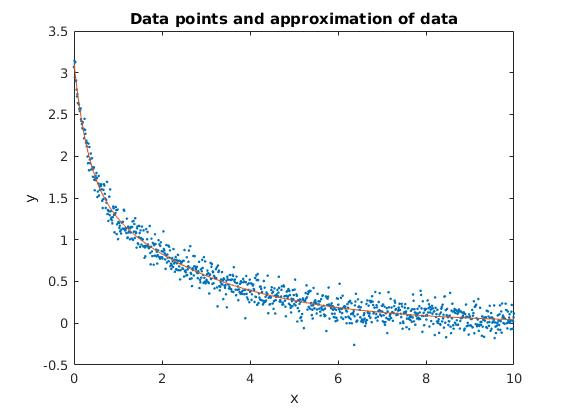
\includegraphics[width=\linewidth,natwidth=610,natheight=642]{ex1_data1.jpg}
	\caption {Data and least square approximatiotn for dataset 'data1'.}
}
%
\parbox[t]{0.4\textwidth}{
	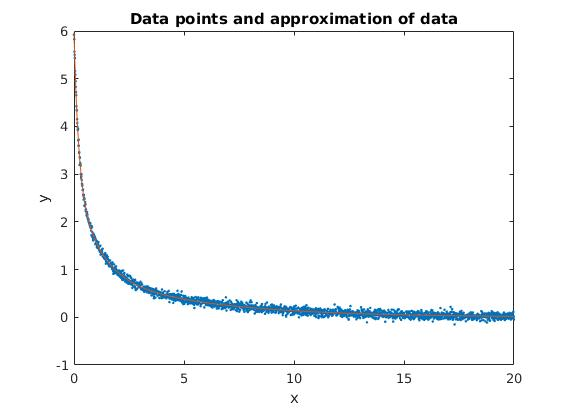
\includegraphics[width=\linewidth,natwidth=610,natheight=642]{ex1_data2.jpg}
	\caption{Data and least square approximatiotn for dataset 'data2'.}
    %\label{cauchy}
}
\hfill
\parbox[t]{0.4\textwidth }{
	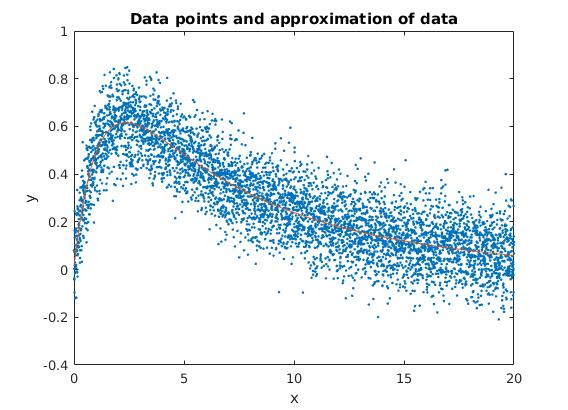
\includegraphics[width =\linewidth,natwidth=610,natheight=642]{ex1_data3.jpg}
	\caption{Data and least square approximatiotn for dataset 'data3'.}
    %\label{logitnormaal}
 }
 \end{figure}
%answers to questions asked in the assignment
%No real questions,only something about values of exp which are 'hidden in signals' and how many???
\section*{Exercise \rom{2}}

%how should the function be called + example
The function Oosterhuis\_assignment3\_exercise2 takes an $n$ number of points. From this points a figure is made by connection the points using interpolation such that a closed curve $C$ is constructed. The function should be called without arguments, a figure with the xy-plane instead will pop up where the user can click the points which will be the coordinates. As an example, the figure of a hand is drawn. The result of the points and the connecting lines is shown in figure \ref{ex2_1}.
\begin{figure}[H]
\centering
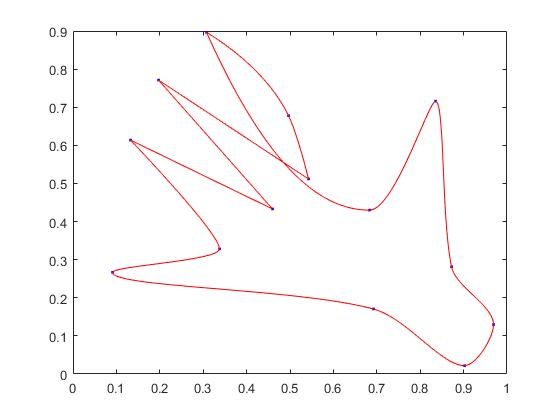
\includegraphics[width=0.6\linewidth,natwidth=610,natheight=642]{ex2_hand.jpg}
%[width=0.6\linewidth]
\caption{}
\label{ex2_1}
\end{figure}

%concise description of the method
To determine the length of C, the cumulative sum of the square root of the elementswise differences of x squared plus the elementwise differences of y squared are taken. Using interpolation between every points $(x_i,y_i)$ and  $(x_{i+1},y_{i+1})$ a line is constucted. The points with the interpolated lines are plotted. The coordinates of the center of mass of the figure are equal to $\bigl((\int_{\Omega}x) / (\int_{\Omega}1); ((\int_{\Omega}x) / (\int_{\Omega}1)\bigr)$.
%short discussion of the reliability and precision of the answer. restrictions program. When does program not work?

%illustration of output and how figure was produced. describe picture
An example of the output of the function is showsn above in \ref{ex2_1}. The picture was produced by taking the points on the xy-plane as defined by the user. The points are stored in two vectors, one with the x-component and one with the y-component of every number. To make a closed curve, both vectors get an extra point at the end of the vector, being the same element as the first one.
%answers to questions asked in the assignment

\section*{Exercise \rom{3}}

%how should the function be called + example
The functions Oosterhuis\_exercise3\_assignment3\_2 calculates the discrete Fourier transform or the inverse discrete Fourier transform of a vector. The function takes zero or a one, a zero indicates the discrete Fourier transform should be calculated and  a one indicates its inverse should be calculated. The second function input is a vector of length $2^n$. This is the vector of which the (inverse) discrete Fourier transform will be calculated. As an example the function is called with the arguments zero and the vector $x = [0;0.707;1;0.707;0;-0.707;-1;-0.707]$. The elements of this vector are values from the $\sin(x), x\in[0,2\pi]$. The output of the function is the vector of the same length as x.

%concise description of the method
The function uses recursion. When the vector is called with a vector of length one, the function output will be just this vector. When the function is called with a vector of length $2^n$, the function will make two vectors: a vector of the even elements and a vector of the odd elements of the original vector. From both these vectors the Fourier transform is calculated using the function Oosterhuis\_exercise3\_assignment3\_2 again with as arguments the new vector and the one or zero unchanged. Note that this is the step where the recursion takes place. After the discrete Fourier transform of the vectors with the even and the odd elements are computed, we call them y\_even respectively y\_odd. The vector y\_even is multiplied with $\omega = \exp(-2 \pi i / N) * v $, where $v$ a is the vector $\begin{bmatrix} 0 \\ 1 \\ \dots \\ N \end{bmatrix} $ and $N$ is the length of both the vectors y\_even and y\_odd. A vector with two elements is created: $y = \begin{bmatrix} y_{odd} + \omega y_{even} \\ y_{odd} - \omega y_{even} \end{bmatrix}$. This vector is the function output and will be the Fourier transform of the given vector.
The inverse discrete Fourier transform is calculated the same way, only using $\omega = \exp{(2\pi i / N)} * \begin{bmatrix} 0 \\ 1 \\ \dots \\N \end{bmatrix}$, so without the minus sign in the exponent. %CHECK DIT

%short discussion of the reliability and precision of the answer. restrictions program. When does program not work?
%
The function does not work whenever the length of the input vector is not a power of two, since at a certain moment in the recursion the length of the vector that needs to be splitted is not even. Another restriction of the function is the fact that it uses the discrete Fourier transform, not the continuous Fourier transform. Hence a function is only being evaluated at a finite number of points, giving an error. %%VERDER UITLEGGEN

%illustration of output and how figure was produced. describe picture
As an example the discrete fourier transform of the function $\sum_{n=1}^{k} n \cos(n\omega t), \omega = 20 \pi$ is computed. This function is plotted in figure \ref{fig3_1}. The discrete Fourier transform of this function is shown in figure \ref{fig3_2}. The discrete Fourier transform is plotted in the fequency domain and shows for each given frequency how much of the signal lies within that frequency. 
The figure of the discrete Fourier transform was produced by evaluating the time function on $128$ points between in the interval $0;0.5]$. From this vector the discrete Fourier transform was computed. This gives a vector of complex numbers. For every complex number the magnitude is calculated. To make the frequencies one sided this was only done for the first half of the vector, the other elements are deleted so this results in a vector of length $64$. To scale the amplitudes, every elements in this vector is devided by $128$, the number of oberservations. This final vector of length $64$ is plotted against a vector with the different frequencies, in this case $1$ to $64$ with stepwidth one.
%figures
\begin{figure}[H]
\centering
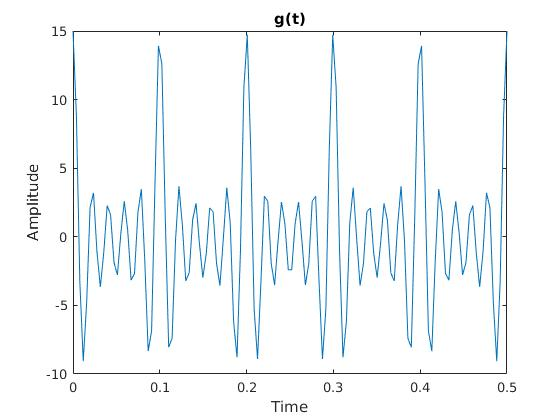
\includegraphics[width=0.6\linewidth,natwidth=610,natheight=642]{ex3_func_wiki_1_func.jpg}
%[width=0.6\linewidth]
\caption{$g(t)= \sum_{n=1}^{k} n \cos(n\omega t), \omega = 20 \pi$}
\label{fig3_1}
\end{figure}
%
%figures
\begin{figure}[H]
\centering
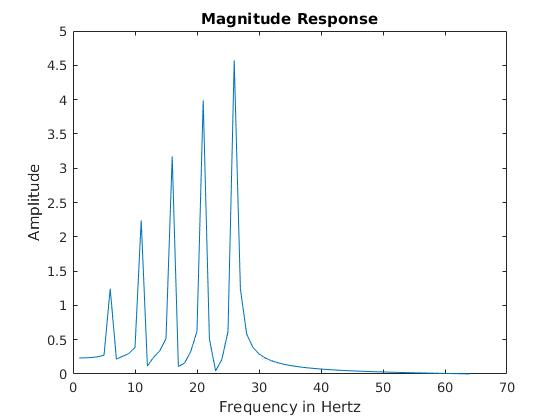
\includegraphics[width=0.6\linewidth,natwidth=610,natheight=642]{ex3_func_wiki_1_four.jpg}
%[width=0.6\linewidth]
\caption{Discrete Fourier transform of $g(t)$ in frequency domain.}
\label{fig3_1}
\end{figure}

%answers to questions asked in the assignment
For large n, the function is not very fast. For the example above, where the function was evaluated at $128$ points, it took about 40 seconds to make the plot. We take a look at the formula for the discrete Fourier transform $F_m = \sum_{k=1}^{N}f_k\omega^{(k-1)(m-1)}$. Since $\omega$ is unknown these are all linear equations so computing the Fourier transform is just matrix multiplication. This implies the number of operations needed is $O(N^2)$, which is way to much to use it for larger datasets. To reduce the number of computations $F_f(m)$ is splitted in a function on the even elements and a function on the odd elements of the input vector: $F_f(m) = F_{f_{odd}}(m) + \omega_{N/2}^{m-1}F_{f_{feven}}(m).$ This allows to interpret $F_{f_{odd/even}}$ as twice repeated vectors. Using this equation the number of operations will reduce to $O(N \log_2 N)$

%convolution
The convolution of two functions $f$ and $g$ evaluated at $2^n$ number of points can be computed by taking the inverse Fourier transform of the product of the Fourier transform of both functions. This method is used in Oosterhuis\_assignment3\_exercise3\_3. This function can take two function handles and will evaluate these functions at eight number of points or the function can take vectors which consist of the evaluation of a function in $2^n$ number of points.
%nog iets over derivatives using fourier, of gewoon weg laten?
%derivates (first and second)
\end{document}
